\documentclass[9pt,letter]{article}
\usepackage{lmodern}
\usepackage{amssymb,amsmath}
\usepackage{ifxetex,ifluatex}
\usepackage{fixltx2e} % provides \textsubscript
\ifnum 0\ifxetex 1\fi\ifluatex 1\fi=0 % if pdftex
  \usepackage[T1]{fontenc}
  \usepackage[utf8]{inputenc}
\else % if luatex or xelatex
  \ifxetex
    \usepackage{mathspec}
  \else
    \usepackage{fontspec}
  \fi
  \defaultfontfeatures{Ligatures=TeX,Scale=MatchLowercase}
\fi
% use upquote if available, for straight quotes in verbatim environments
\IfFileExists{upquote.sty}{\usepackage{upquote}}{}
% use microtype if available
\IfFileExists{microtype.sty}{%
\usepackage{microtype}
\UseMicrotypeSet[protrusion]{basicmath} % disable protrusion for tt fonts
}{}
\usepackage[margin=.75in]{geometry}
\usepackage{hyperref}
\hypersetup{unicode=true,
            pdftitle={Assignment 4},
            pdfauthor={Azoacha Forcheh, 20558994},
            pdfborder={0 0 0},
            breaklinks=true}
\urlstyle{same}  % don't use monospace font for urls
\usepackage{color}
\usepackage{fancyvrb}
\newcommand{\VerbBar}{|}
\newcommand{\VERB}{\Verb[commandchars=\\\{\}]}
\DefineVerbatimEnvironment{Highlighting}{Verbatim}{commandchars=\\\{\}}
% Add ',fontsize=\small' for more characters per line
\usepackage{framed}
\definecolor{shadecolor}{RGB}{248,248,248}
\newenvironment{Shaded}{\begin{snugshade}}{\end{snugshade}}
\newcommand{\KeywordTok}[1]{\textcolor[rgb]{0.13,0.29,0.53}{\textbf{#1}}}
\newcommand{\DataTypeTok}[1]{\textcolor[rgb]{0.13,0.29,0.53}{#1}}
\newcommand{\DecValTok}[1]{\textcolor[rgb]{0.00,0.00,0.81}{#1}}
\newcommand{\BaseNTok}[1]{\textcolor[rgb]{0.00,0.00,0.81}{#1}}
\newcommand{\FloatTok}[1]{\textcolor[rgb]{0.00,0.00,0.81}{#1}}
\newcommand{\ConstantTok}[1]{\textcolor[rgb]{0.00,0.00,0.00}{#1}}
\newcommand{\CharTok}[1]{\textcolor[rgb]{0.31,0.60,0.02}{#1}}
\newcommand{\SpecialCharTok}[1]{\textcolor[rgb]{0.00,0.00,0.00}{#1}}
\newcommand{\StringTok}[1]{\textcolor[rgb]{0.31,0.60,0.02}{#1}}
\newcommand{\VerbatimStringTok}[1]{\textcolor[rgb]{0.31,0.60,0.02}{#1}}
\newcommand{\SpecialStringTok}[1]{\textcolor[rgb]{0.31,0.60,0.02}{#1}}
\newcommand{\ImportTok}[1]{#1}
\newcommand{\CommentTok}[1]{\textcolor[rgb]{0.56,0.35,0.01}{\textit{#1}}}
\newcommand{\DocumentationTok}[1]{\textcolor[rgb]{0.56,0.35,0.01}{\textbf{\textit{#1}}}}
\newcommand{\AnnotationTok}[1]{\textcolor[rgb]{0.56,0.35,0.01}{\textbf{\textit{#1}}}}
\newcommand{\CommentVarTok}[1]{\textcolor[rgb]{0.56,0.35,0.01}{\textbf{\textit{#1}}}}
\newcommand{\OtherTok}[1]{\textcolor[rgb]{0.56,0.35,0.01}{#1}}
\newcommand{\FunctionTok}[1]{\textcolor[rgb]{0.00,0.00,0.00}{#1}}
\newcommand{\VariableTok}[1]{\textcolor[rgb]{0.00,0.00,0.00}{#1}}
\newcommand{\ControlFlowTok}[1]{\textcolor[rgb]{0.13,0.29,0.53}{\textbf{#1}}}
\newcommand{\OperatorTok}[1]{\textcolor[rgb]{0.81,0.36,0.00}{\textbf{#1}}}
\newcommand{\BuiltInTok}[1]{#1}
\newcommand{\ExtensionTok}[1]{#1}
\newcommand{\PreprocessorTok}[1]{\textcolor[rgb]{0.56,0.35,0.01}{\textit{#1}}}
\newcommand{\AttributeTok}[1]{\textcolor[rgb]{0.77,0.63,0.00}{#1}}
\newcommand{\RegionMarkerTok}[1]{#1}
\newcommand{\InformationTok}[1]{\textcolor[rgb]{0.56,0.35,0.01}{\textbf{\textit{#1}}}}
\newcommand{\WarningTok}[1]{\textcolor[rgb]{0.56,0.35,0.01}{\textbf{\textit{#1}}}}
\newcommand{\AlertTok}[1]{\textcolor[rgb]{0.94,0.16,0.16}{#1}}
\newcommand{\ErrorTok}[1]{\textcolor[rgb]{0.64,0.00,0.00}{\textbf{#1}}}
\newcommand{\NormalTok}[1]{#1}
\usepackage{graphicx,grffile}
\makeatletter
\def\maxwidth{\ifdim\Gin@nat@width>\linewidth\linewidth\else\Gin@nat@width\fi}
\def\maxheight{\ifdim\Gin@nat@height>\textheight\textheight\else\Gin@nat@height\fi}
\makeatother
% Scale images if necessary, so that they will not overflow the page
% margins by default, and it is still possible to overwrite the defaults
% using explicit options in \includegraphics[width, height, ...]{}
\setkeys{Gin}{width=\maxwidth,height=\maxheight,keepaspectratio}
\IfFileExists{parskip.sty}{%
\usepackage{parskip}
}{% else
\setlength{\parindent}{0pt}
\setlength{\parskip}{6pt plus 2pt minus 1pt}
}
\setlength{\emergencystretch}{3em}  % prevent overfull lines
\providecommand{\tightlist}{%
  \setlength{\itemsep}{0pt}\setlength{\parskip}{0pt}}
\setcounter{secnumdepth}{0}
% Redefines (sub)paragraphs to behave more like sections
\ifx\paragraph\undefined\else
\let\oldparagraph\paragraph
\renewcommand{\paragraph}[1]{\oldparagraph{#1}\mbox{}}
\fi
\ifx\subparagraph\undefined\else
\let\oldsubparagraph\subparagraph
\renewcommand{\subparagraph}[1]{\oldsubparagraph{#1}\mbox{}}
\fi

%%% Use protect on footnotes to avoid problems with footnotes in titles
\let\rmarkdownfootnote\footnote%
\def\footnote{\protect\rmarkdownfootnote}

%%% Change title format to be more compact
\usepackage{titling}

% Create subtitle command for use in maketitle
\newcommand{\subtitle}[1]{
  \posttitle{
    \begin{center}\large#1\end{center}
    }
}

\setlength{\droptitle}{-2em}
  \title{Assignment 4}
  \pretitle{\vspace{\droptitle}\centering\huge}
  \posttitle{\par}
  \author{Azoacha Forcheh, 20558994}
  \preauthor{\centering\large\emph}
  \postauthor{\par}
  \date{}
  \predate{}\postdate{}

\usepackage{graphicx}
\usepackage{color}
\usepackage{enumitem}
\newcommand{\benum}{\begin{enumerate}}
\newcommand{\eenum}{\end{enumerate}}
\newcommand{\bitem}{\begin{itemize}}
\newcommand{\eitem}{\end{itemize}}

\begin{document}
\maketitle

\benum
\item Download the \texttt{diabetes} data from the course website. In
that file, there is a dataset on various measurements of 145 patients.
Once you load this file into your R session (or equivalently, execute
its contents there) there will be a data set called \texttt{diabetes}.

The variate \texttt{SSPG} stands for steady state plasma glucose which
measures the patient's insulin resistance, a pathological condition
where the body's cells fail to respond to the hormone insulin.

\benum
\item (3 marks) Produce a plot of a density estimate of \texttt{SSPG}
and comment on what you see.

\begin{Shaded}
\begin{Highlighting}[]
\CommentTok{# Should I stretch out the limits so that this doesn't look cut off?}
\KeywordTok{library}\NormalTok{(ggplot2)}
\NormalTok{sspg_plot =}\StringTok{ }\KeywordTok{ggplot}\NormalTok{(}\DataTypeTok{data =}\NormalTok{ diabetes, }\DataTypeTok{mapping =} \KeywordTok{aes}\NormalTok{(}\DataTypeTok{x=}\NormalTok{SSPG))}
\NormalTok{sspg_plot }\OperatorTok{+}
\StringTok{  }\KeywordTok{geom_density}\NormalTok{(}\DataTypeTok{colour=}\StringTok{"grey50"}\NormalTok{, }\DataTypeTok{fill=}\StringTok{"grey50"}\NormalTok{, }\DataTypeTok{bw=}\StringTok{"SJ"}\NormalTok{) }\OperatorTok{+}
\StringTok{  }\KeywordTok{scale_x_continuous}\NormalTok{(}\DataTypeTok{limits=}\KeywordTok{c}\NormalTok{(}\OperatorTok{-}\DecValTok{100}\NormalTok{, }\DecValTok{600}\NormalTok{))}
\end{Highlighting}
\end{Shaded}

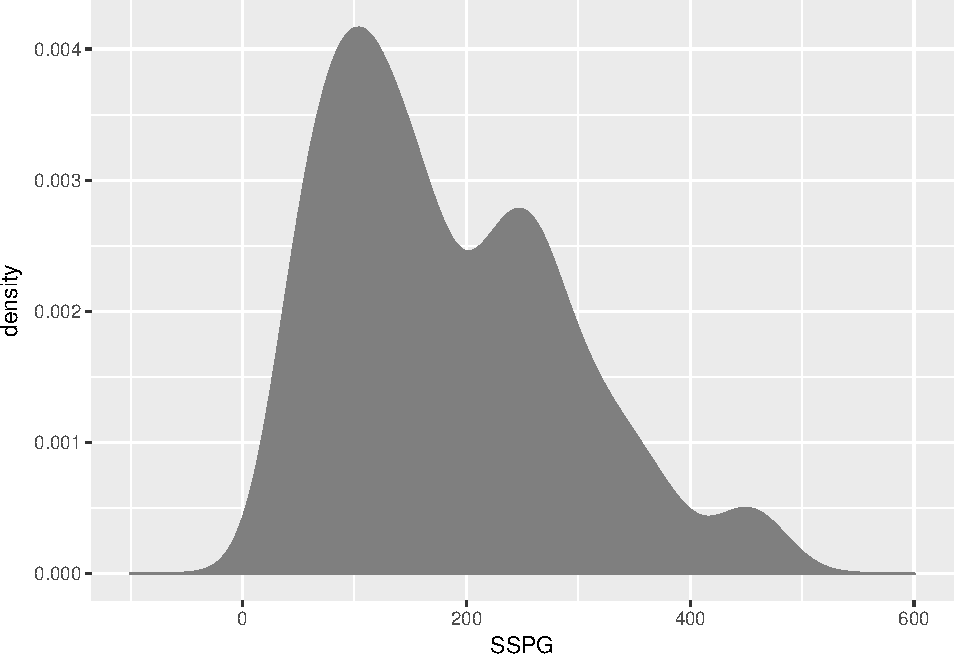
\includegraphics{a4_testing_files/figure-latex/unnamed-chunk-2-1.pdf}

\begin{Shaded}
\begin{Highlighting}[]
\NormalTok{sspg_dens =}\StringTok{ }\KeywordTok{density}\NormalTok{(diabetes}\OperatorTok{$}\NormalTok{SSPG, }\DataTypeTok{bw=}\StringTok{"SJ"}\NormalTok{)}
\KeywordTok{plot}\NormalTok{(sspg_dens, }\DataTypeTok{main=}\StringTok{"Density Estimate of SSPG Measurements"}\NormalTok{)}
\KeywordTok{polygon}\NormalTok{(sspg_dens, }\DataTypeTok{col=}\StringTok{"dark grey"}\NormalTok{, }\DataTypeTok{border=}\StringTok{"dark grey"}\NormalTok{, }\DataTypeTok{xlab=}\StringTok{"SSPG"}\NormalTok{)}
\end{Highlighting}
\end{Shaded}

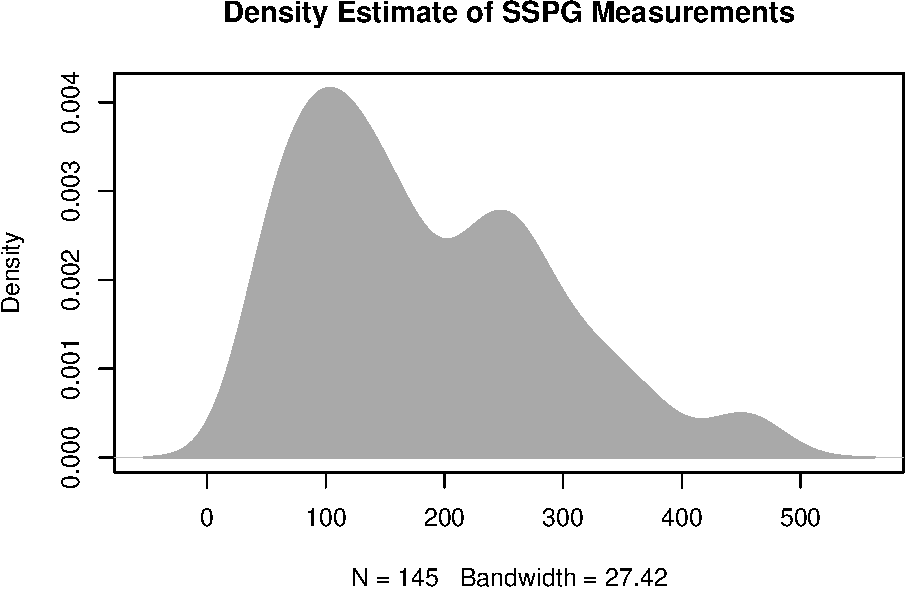
\includegraphics{a4_testing_files/figure-latex/unnamed-chunk-3-1.pdf}

The density is right-skewed and trimodal, with modes at about 100, 250
and 450. The curve rises quickly to the first mode, then gradually
decreases. In addition, the majority of patients have an SSG measurement
below 250. Lastly, the SSPG seems lacks normality - i.e.~it does not
seem to have been sampled from the normal - as its density does not
resemble the symmetric bell curve of a normal density.

\item 

Construct a quantile plot of \texttt{SSPG} and comment on the shape of
its distribution.

\begin{Shaded}
\begin{Highlighting}[]
\NormalTok{sspg_vals =}\StringTok{ }\KeywordTok{sort}\NormalTok{(diabetes}\OperatorTok{$}\NormalTok{SSPG)}
\NormalTok{n =}\StringTok{ }\KeywordTok{length}\NormalTok{(sspg_vals)}
\NormalTok{p =}\StringTok{ }\KeywordTok{ppoints}\NormalTok{(n) }\CommentTok{# the proportions}

\KeywordTok{plot}\NormalTok{(}\DataTypeTok{x =}\NormalTok{ p, }\DataTypeTok{y =}\NormalTok{ sspg_vals, }\DataTypeTok{type=}\StringTok{"o"}\NormalTok{, }\DataTypeTok{lwd=}\DecValTok{2}\NormalTok{, }\DataTypeTok{col=}\StringTok{"grey10"}\NormalTok{,}
    \DataTypeTok{xlab=}\StringTok{"cumulative proportion"}\NormalTok{, }\DataTypeTok{xlim=}\KeywordTok{c}\NormalTok{(}\DecValTok{0}\NormalTok{,}\DecValTok{1}\NormalTok{),}
    \DataTypeTok{ylab=}\StringTok{"SSPG"}\NormalTok{, }\DataTypeTok{main=}\StringTok{"Quantile Plot of SSPG Measurements"}\NormalTok{)}
\end{Highlighting}
\end{Shaded}

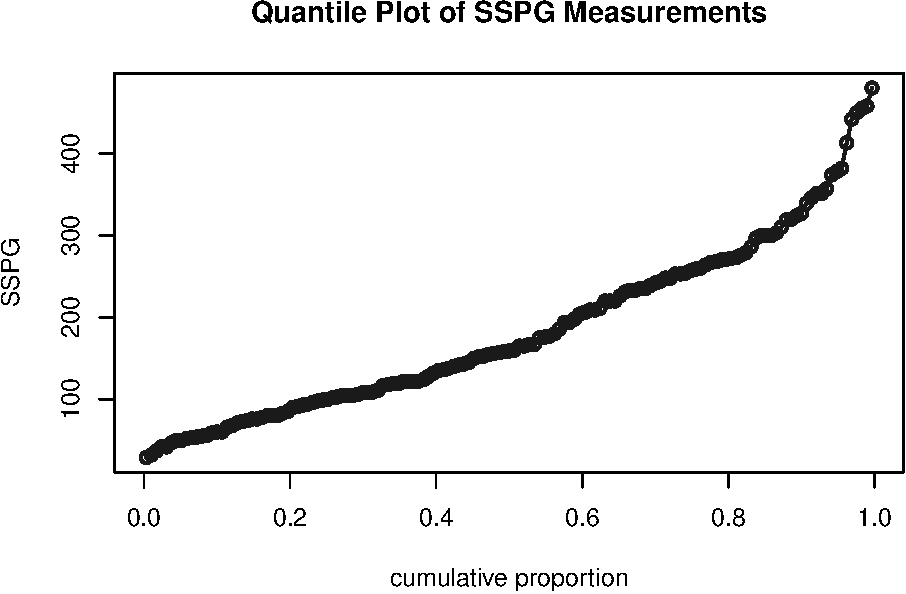
\includegraphics{a4_testing_files/figure-latex/unnamed-chunk-4-1.pdf}

The shape of the quantile plot is nearly linear up until about the 60th
percentile, at which point it begins to curve upwards. The data seems to
be evenly concentraed throughout the plot, with sparsity at the right
tail. This indicates a lot of variation between the extremes as the
concentration of points at the left tail of the plot is relatively
higher. Overall, the plot has a convex, trough-down shape.

\item 

(3 marks) Use \texttt{qqtest} to construct a qqplot that compares
\texttt{SSPG} to a standard normal distribution. Include envelopes in
the plot. Comment on the distribution of \texttt{SSPG} and whether it
might reasonably be regarded as a sample from some normal distribution.
Explain your reasoning.

\textbf{Important:} Before every \texttt{qqtest} execute
\texttt{set.seed(3124159)} so that we are all seeing the same plots.

\begin{Shaded}
\begin{Highlighting}[]
\KeywordTok{library}\NormalTok{(qqtest)}
\CommentTok{# Setting the seed}
\CommentTok{# See page 57 of Part 3 of Comparing Distributions for commentary info}
\KeywordTok{set.seed}\NormalTok{(}\DecValTok{3124159}\NormalTok{)}
\KeywordTok{qqtest}\NormalTok{(}\DataTypeTok{data=}\NormalTok{diabetes}\OperatorTok{$}\NormalTok{SSPG)}
\end{Highlighting}
\end{Shaded}

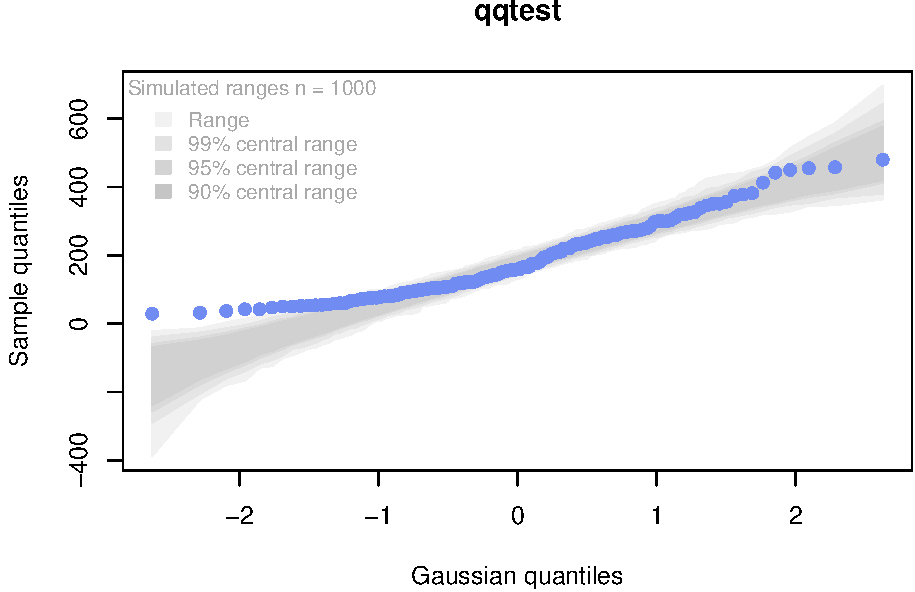
\includegraphics{a4_testing_files/figure-latex/unnamed-chunk-5-1.pdf}

\item 

The last variate, \texttt{ClinClass}, represents the classification of
each patient according to the 1979 medical criteria into one of three
groups: 1 = ``Overt Diabetic'', 2 = ``Chemical Diabetic'', and 3 =
``Normal''.

\benum     \item (4 marks) Construct a back to back density line-up plot
to assess whether the normal and diabetic (chemical and overt combined)
\texttt{SSPG} values come from the same distribution. Use
\texttt{set.seed(3124159)} and show your code. What conclusions do you
draw?

\begin{Shaded}
\begin{Highlighting}[]
\NormalTok{normal_SSPG =}\StringTok{ }\NormalTok{diabetes[diabetes}\OperatorTok{$}\NormalTok{ClinClass }\OperatorTok{==}\StringTok{ }\DecValTok{3}\NormalTok{,]}\OperatorTok{$}\NormalTok{SSPG}
\NormalTok{diabetic_SSPG =}\StringTok{ }\NormalTok{diabetes[diabetes}\OperatorTok{$}\NormalTok{ClinClass }\OperatorTok{!=}\StringTok{ }\DecValTok{3}\NormalTok{,]}\OperatorTok{$}\NormalTok{SSPG}

\NormalTok{back2back <-}\StringTok{ }\ControlFlowTok{function}\NormalTok{(data, suspectNo) \{}
\NormalTok{  ylim =}\StringTok{ }\KeywordTok{extendrange}\NormalTok{(}\KeywordTok{c}\NormalTok{(data}\OperatorTok{$}\NormalTok{x, data}\OperatorTok{$}\NormalTok{y)) }\CommentTok{#c(0,600)}
\NormalTok{  Xdensity =}\StringTok{ }\KeywordTok{density}\NormalTok{(data}\OperatorTok{$}\NormalTok{x, }\DataTypeTok{bw=}\StringTok{"SJ"}\NormalTok{)}
\NormalTok{  Ydensity =}\StringTok{ }\KeywordTok{density}\NormalTok{(data}\OperatorTok{$}\NormalTok{y, }\DataTypeTok{bw=}\StringTok{"SJ"}\NormalTok{)}
\NormalTok{  Ydensity}\OperatorTok{$}\NormalTok{y =}\StringTok{ }\OperatorTok{-}\NormalTok{Ydensity}\OperatorTok{$}\NormalTok{y}
\NormalTok{  xlim =}\StringTok{ }\KeywordTok{extendrange}\NormalTok{(}\KeywordTok{c}\NormalTok{(Xdensity}\OperatorTok{$}\NormalTok{y, Ydensity}\OperatorTok{$}\NormalTok{y))}
  
\NormalTok{  xyswitch <-}\StringTok{ }\ControlFlowTok{function}\NormalTok{(xy_plot) \{}
\NormalTok{    yx_plot =}\StringTok{ }\NormalTok{xy_plot}
\NormalTok{    yx_plot}\OperatorTok{$}\NormalTok{x =}\StringTok{ }\NormalTok{xy_plot}\OperatorTok{$}\NormalTok{y}
\NormalTok{    yx_plot}\OperatorTok{$}\NormalTok{y =}\StringTok{ }\NormalTok{xy_plot}\OperatorTok{$}\NormalTok{x}
\NormalTok{    yx_plot}
\NormalTok{  \}}
  
  \KeywordTok{plot}\NormalTok{(}\KeywordTok{xyswitch}\NormalTok{(Xdensity), }\DataTypeTok{col=}\StringTok{"firebrick"}\NormalTok{,}
       \DataTypeTok{xlab=}\StringTok{""}\NormalTok{, }\DataTypeTok{ylab=}\StringTok{""}\NormalTok{, }\DataTypeTok{xaxt=}\StringTok{"n"}\NormalTok{, }\DataTypeTok{yaxt=}\StringTok{"n"}\NormalTok{,}
       \DataTypeTok{main=}\KeywordTok{paste}\NormalTok{(}\StringTok{"i = "}\NormalTok{, suspectNo),}\CommentTok{# display suspect number}
       \DataTypeTok{cex.main =} \DecValTok{2}\NormalTok{, }\CommentTok{# increase suspect number size}
       \DataTypeTok{xlim=}\NormalTok{xlim, }\DataTypeTok{ylim=}\NormalTok{ylim)}
  \KeywordTok{polygon}\NormalTok{(}\KeywordTok{xyswitch}\NormalTok{(Xdensity), }\DataTypeTok{col=}\KeywordTok{adjustcolor}\NormalTok{(}\StringTok{"firebrick"}\NormalTok{, }\FloatTok{0.4}\NormalTok{))}
  \KeywordTok{lines}\NormalTok{(}\KeywordTok{xyswitch}\NormalTok{(Ydensity), }\DataTypeTok{col=}\StringTok{"steelblue"}\NormalTok{)}
  \KeywordTok{polygon}\NormalTok{(}\KeywordTok{xyswitch}\NormalTok{(Ydensity), }\DataTypeTok{col=}\KeywordTok{adjustcolor}\NormalTok{(}\StringTok{"steelblue"}\NormalTok{,}\FloatTok{0.4}\NormalTok{))}
\NormalTok{\}}

\NormalTok{mixRandomly <-}\StringTok{ }\ControlFlowTok{function}\NormalTok{(data) \{}
  \CommentTok{# Note that data need not be a data frame}
  \CommentTok{# It is expected to be a list with an x and a y component}
  \CommentTok{# (possibly of different lengths)}
\NormalTok{  x <-}\StringTok{ }\NormalTok{data}\OperatorTok{$}\NormalTok{x}
\NormalTok{  y <-}\StringTok{ }\NormalTok{data}\OperatorTok{$}\NormalTok{y}
\NormalTok{  n_x <-}\KeywordTok{length}\NormalTok{(x)}
\NormalTok{  n_y <-}\KeywordTok{length}\NormalTok{(y)}
\NormalTok{  mix <-}\KeywordTok{c}\NormalTok{(x,y)}
\NormalTok{  select4x <-}\KeywordTok{sample}\NormalTok{(}\DecValTok{1}\OperatorTok{:}\NormalTok{(n_x}\OperatorTok{+}\NormalTok{n_y),n_x,}\DataTypeTok{replace =} \OtherTok{FALSE}\NormalTok{)}
\NormalTok{  new_x <-}\StringTok{ }\NormalTok{mix[select4x] }\CommentTok{# The mixing occurs}
\NormalTok{  new_y <-}\StringTok{ }\NormalTok{mix[}\OperatorTok{-}\NormalTok{select4x]}
  \KeywordTok{list}\NormalTok{(}\DataTypeTok{x=}\NormalTok{new_x, }\DataTypeTok{y=}\NormalTok{new_y)}
\NormalTok{\}}

\NormalTok{lineup <-}\StringTok{ }\ControlFlowTok{function}\NormalTok{(data, }\DataTypeTok{showSuspect=}\OtherTok{NULL}\NormalTok{, }\DataTypeTok{generateSuspect=}\OtherTok{NULL}\NormalTok{,}
                   \DataTypeTok{trueLoc=}\OtherTok{NULL}\NormalTok{, }\DataTypeTok{layout =}\KeywordTok{c}\NormalTok{(}\DecValTok{5}\NormalTok{,}\DecValTok{4}\NormalTok{)) \{}
  \CommentTok{# Get the number of suspects in total}
\NormalTok{  nSuspects <-}\StringTok{ }\NormalTok{layout[}\DecValTok{1}\NormalTok{] }\OperatorTok{*}\StringTok{ }\NormalTok{layout[}\DecValTok{2}\NormalTok{]}
  \ControlFlowTok{if}\NormalTok{ (}\KeywordTok{is.null}\NormalTok{(trueLoc)) \{trueLoc <-}\KeywordTok{sample}\NormalTok{(}\DecValTok{1}\OperatorTok{:}\NormalTok{nSuspects, }\DecValTok{1}\NormalTok{)\}}
  \ControlFlowTok{if}\NormalTok{ (}\KeywordTok{is.null}\NormalTok{(showSuspect)) \{}\KeywordTok{stop}\NormalTok{(}\StringTok{"need a plot function for the suspect"}\NormalTok{)\}}
  \ControlFlowTok{if}\NormalTok{ (}\KeywordTok{is.null}\NormalTok{(generateSuspect)) \{}\KeywordTok{stop}\NormalTok{(}\StringTok{"need a function to generate suspect"}\NormalTok{)\}}
  \CommentTok{# Need to decide which subject to present}
\NormalTok{  presentSuspect <-}\StringTok{ }\ControlFlowTok{function}\NormalTok{(suspectNo) \{}
    \ControlFlowTok{if}\NormalTok{(suspectNo }\OperatorTok{!=}\StringTok{ }\NormalTok{trueLoc) \{data <-}\KeywordTok{generateSuspect}\NormalTok{(data)\}}
    \KeywordTok{showSuspect}\NormalTok{(data, suspectNo) }
\NormalTok{  \}}
  \CommentTok{# This does the plotting}
\NormalTok{  savePar <-}\KeywordTok{par}\NormalTok{(}\DataTypeTok{mfrow=}\NormalTok{layout,}\DataTypeTok{mar=}\KeywordTok{c}\NormalTok{(}\FloatTok{2.5}\NormalTok{, }\FloatTok{0.1}\NormalTok{, }\DecValTok{3}\NormalTok{, }\FloatTok{0.1}\NormalTok{), }\DataTypeTok{oma=}\KeywordTok{rep}\NormalTok{(}\DecValTok{0}\NormalTok{,}\DecValTok{4}\NormalTok{))}
  \KeywordTok{sapply}\NormalTok{(}\DecValTok{1}\OperatorTok{:}\NormalTok{nSuspects, }\DataTypeTok{FUN =}\NormalTok{ presentSuspect)}
  \KeywordTok{par}\NormalTok{(savePar)}
  
  \CommentTok{# Obfuscate location to keep us honest}
\NormalTok{  possibleBaseVals <-}\StringTok{ }\DecValTok{3}\OperatorTok{:}\KeywordTok{min}\NormalTok{(}\DecValTok{2}\OperatorTok{*}\NormalTok{nSuspects, }\DecValTok{50}\NormalTok{) }\CommentTok{# remove easy base values}
\NormalTok{  possibleBaseVals <-}\StringTok{ }\NormalTok{possibleBaseVals[possibleBaseVals }\OperatorTok{!=}\StringTok{ }\DecValTok{10} \OperatorTok{&}\StringTok{ }\NormalTok{possibleBaseVals }\OperatorTok{!=}\StringTok{ }\DecValTok{5}\NormalTok{]}
\NormalTok{  base <-}\KeywordTok{sample}\NormalTok{(possibleBaseVals, }\DecValTok{1}\NormalTok{)}
\NormalTok{  offset <-}\KeywordTok{sample}\NormalTok{(}\DecValTok{5}\OperatorTok{:}\KeywordTok{min}\NormalTok{(}\DecValTok{5}\OperatorTok{*}\NormalTok{nSuspects, }\DecValTok{125}\NormalTok{),}\DecValTok{1}\NormalTok{)}
  
  \CommentTok{# return obfuscated location}
  \KeywordTok{list}\NormalTok{(}\DataTypeTok{trueLoc =}\KeywordTok{paste0}\NormalTok{(}\StringTok{"log("}\NormalTok{,base}\OperatorTok{^}\NormalTok{(trueLoc }\OperatorTok{+}\StringTok{ }\NormalTok{offset),}
                       \StringTok{", base="}\NormalTok{,base,}\StringTok{") - "}\NormalTok{, offset))}
\NormalTok{\}}

\NormalTok{data =}\StringTok{ }\KeywordTok{list}\NormalTok{(}\DataTypeTok{x=}\NormalTok{normal_SSPG, }\DataTypeTok{y=}\NormalTok{diabetic_SSPG)}
\KeywordTok{set.seed}\NormalTok{(}\DecValTok{3124159}\NormalTok{)}
\KeywordTok{lineup}\NormalTok{(data,}
       \DataTypeTok{generateSuspect =}\NormalTok{ mixRandomly,}
       \DataTypeTok{showSuspect =}\NormalTok{ back2back)}
\end{Highlighting}
\end{Shaded}

\begin{center}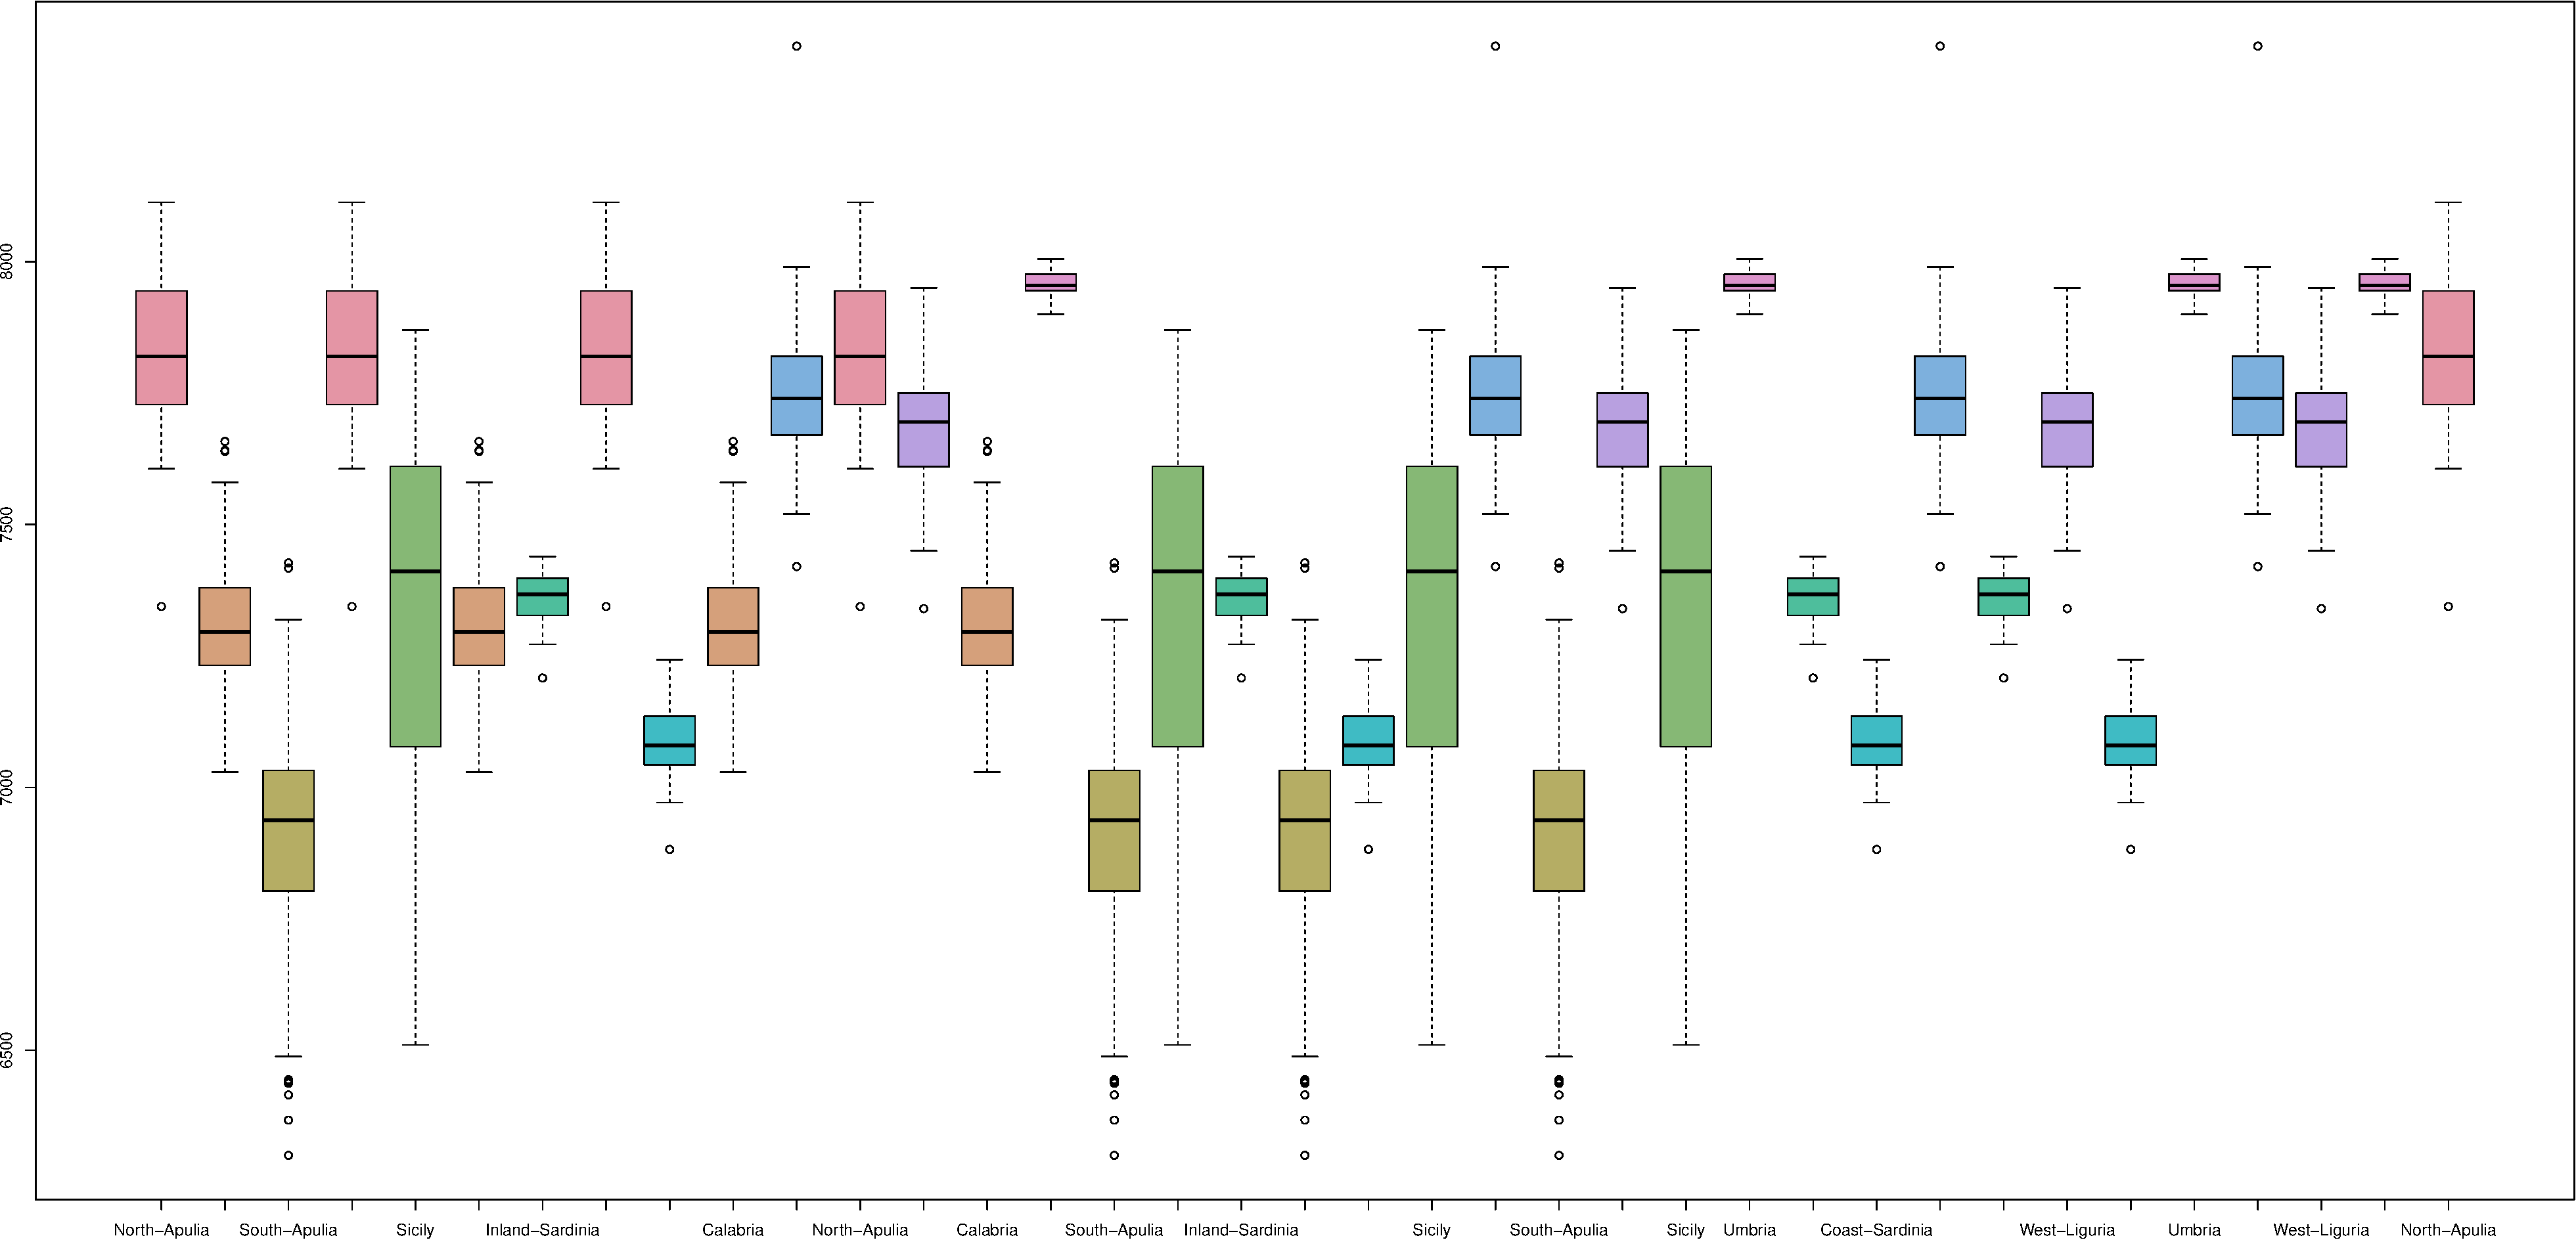
\includegraphics{a4_testing_files/figure-latex/unnamed-chunk-6-1} \end{center}

\begin{verbatim}
## $trueLoc
## [1] "log(7.51141330201283e+30, base=22) - 17"
\end{verbatim}

From the lineup test, it is visually clear that the true plot is at
\(i = 6\) - which is indeed equal to the generated value of
\texttt{trueLoc} - as this plot stands out more than any of the others.
Hence, using this lineup test, there is enough evidence to reject the
hypothesis that the two sets come from the same-shaped distribution.

\item 

(4 marks) Use \texttt{qqtest} to construct a lineup plot making the same
assessment, but this time assess whether the overt diabetic values of
\texttt{SSPG} might have been generated from the same distribution as
the normal patients. Use \texttt{set.seed(3124159)} and show your code.
What conclusions do you draw?

\begin{Shaded}
\begin{Highlighting}[]
\CommentTok{# See page 57 of Part 3 of Comparing Distributions for commentary info}
\KeywordTok{set.seed}\NormalTok{(}\DecValTok{3124159}\NormalTok{)}
\NormalTok{overt_SSPG =}\StringTok{ }\NormalTok{diabetes[diabetes}\OperatorTok{$}\NormalTok{ClinClass }\OperatorTok{==}\StringTok{ }\DecValTok{1}\NormalTok{,]}\OperatorTok{$}\NormalTok{SSPG}
\KeywordTok{qqtest}\NormalTok{(}\DataTypeTok{data =}\NormalTok{ overt_SSPG, }\DataTypeTok{dataTest=}\NormalTok{normal_SSPG,}
       \DataTypeTok{main=}\StringTok{"Testing if Overt diabetic values of SSPG from Normal patients"}\NormalTok{)}
\end{Highlighting}
\end{Shaded}

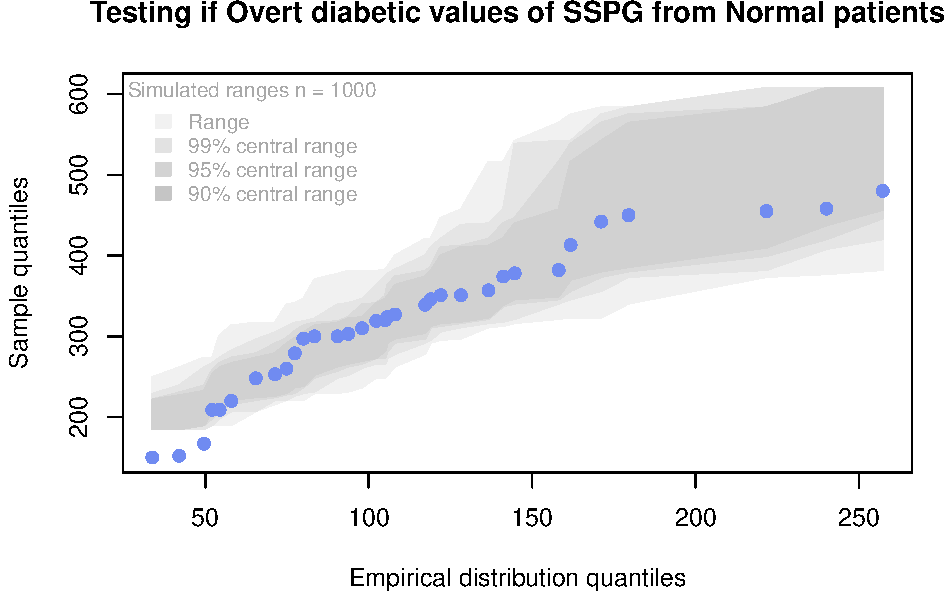
\includegraphics{a4_testing_files/figure-latex/unnamed-chunk-7-1.pdf}

Most of the points in the plot lie within the envolepe, with a few at
the left tail sitting outside the envelope. Hence, there is not enough
evidence to reject the hypothesis that the overt diabetic values of
\texttt{SSPG} might have been generated from the same distribution as
the normal patients.

\item 

\textbf{Grad students, bonus undergraduates} (8 marks) Consider the
following code:

\begin{Shaded}
\begin{Highlighting}[]
\NormalTok{data <-}\StringTok{ }\KeywordTok{list}\NormalTok{(}\DataTypeTok{x=}\NormalTok{x, }\DataTypeTok{y=}\NormalTok{y, }\DataTypeTok{z=}\NormalTok{z)}
\KeywordTok{lineup}\NormalTok{(data, }
\DataTypeTok{generateSuspect =}\NormalTok{ mixRandomly, }
\DataTypeTok{showSuspect =}\NormalTok{ myQuantilePlot, }
\DataTypeTok{layout=}\KeywordTok{c}\NormalTok{(}\DecValTok{5}\NormalTok{,}\DecValTok{4}\NormalTok{))}
\end{Highlighting}
\end{Shaded}

The function \texttt{mixRandomly} will need to be rewritten to handle
\texttt{data} being a list of three samples. Write the function
\texttt{myQuantilePlot} so that it overlays the sample quantile
functions of each of \texttt{x}, \texttt{y}, and \texttt{z} in the same
display using different colours. Hand in your code for these two
functions and illustrate the outcome (using \texttt{set.seed(314159)})
on \texttt{SSPG} for the three different clinical classes. Comment on
your findings.

\begin{Shaded}
\begin{Highlighting}[]
\NormalTok{mixRandomly <-}\StringTok{ }\ControlFlowTok{function}\NormalTok{(data) \{}
  \CommentTok{# Note that data need not be a data frame}
  \CommentTok{# It is expected to be a list with an x, a y and a z component}
  \CommentTok{# (possibly of different lengths)}
\NormalTok{  x =}\StringTok{ }\NormalTok{data}\OperatorTok{$}\NormalTok{x}
\NormalTok{  y =}\StringTok{ }\NormalTok{data}\OperatorTok{$}\NormalTok{y}
\NormalTok{  z =}\StringTok{ }\NormalTok{data}\OperatorTok{$}\NormalTok{z}
\NormalTok{  n_x =}\StringTok{ }\KeywordTok{length}\NormalTok{(x)}
\NormalTok{  n_y =}\StringTok{ }\KeywordTok{length}\NormalTok{(y)}
\NormalTok{  n_z =}\StringTok{ }\KeywordTok{length}\NormalTok{(y)}
\NormalTok{  mix =}\StringTok{ }\KeywordTok{c}\NormalTok{(x,y,z)}
\NormalTok{  full_range =}\StringTok{ }\DecValTok{1}\OperatorTok{:}\NormalTok{(n_x}\OperatorTok{+}\NormalTok{n_y}\OperatorTok{+}\NormalTok{n_z)}
\NormalTok{  select4x =}\StringTok{ }\KeywordTok{sample}\NormalTok{(full_range,n_x,}\DataTypeTok{replace =} \OtherTok{FALSE}\NormalTok{)}
  \CommentTok{# remove indices in select4x from sampling pool and sample indices for y}
\NormalTok{  select4y =}\StringTok{ }\KeywordTok{sample}\NormalTok{(full_range[}\OperatorTok{-}\NormalTok{select4x],n_y,}\DataTypeTok{replace =} \OtherTok{FALSE}\NormalTok{)}
\NormalTok{  new_x =}\StringTok{ }\NormalTok{mix[select4x] }\CommentTok{# The mixing occurs}
\NormalTok{  new_y =}\StringTok{ }\NormalTok{mix[select4y]}
\NormalTok{  new_z =}\StringTok{ }\NormalTok{mix[}\OperatorTok{-}\NormalTok{select4y] }
  \KeywordTok{list}\NormalTok{(}\DataTypeTok{x=}\NormalTok{new_x, }\DataTypeTok{y=}\NormalTok{new_y, }\DataTypeTok{z=}\NormalTok{new_z)}
\NormalTok{\}}

\CommentTok{# should there be an option to specify colors or can we choose any?}
\NormalTok{myQuantilePlot <-}\StringTok{ }\ControlFlowTok{function}\NormalTok{(data, suspectNo) \{}
\NormalTok{  ylim =}\StringTok{ }\KeywordTok{extendrange}\NormalTok{(}\KeywordTok{c}\NormalTok{(data}\OperatorTok{$}\NormalTok{x, data}\OperatorTok{$}\NormalTok{y, data}\OperatorTok{$}\NormalTok{z))}
\NormalTok{  n_x =}\StringTok{ }\KeywordTok{length}\NormalTok{(data}\OperatorTok{$}\NormalTok{x)}
\NormalTok{  n_y =}\StringTok{ }\KeywordTok{length}\NormalTok{(data}\OperatorTok{$}\NormalTok{y)}
\NormalTok{  n_z =}\StringTok{ }\KeywordTok{length}\NormalTok{(data}\OperatorTok{$}\NormalTok{z)}
\NormalTok{  p_x =}\StringTok{ }\KeywordTok{ppoints}\NormalTok{(n_x)}
\NormalTok{  p_y =}\StringTok{ }\KeywordTok{ppoints}\NormalTok{(n_y)}
\NormalTok{  p_z =}\StringTok{ }\KeywordTok{ppoints}\NormalTok{(n_z)}
  \KeywordTok{plot}\NormalTok{(p_x, }\KeywordTok{sort}\NormalTok{(data}\OperatorTok{$}\NormalTok{x), }\DataTypeTok{type=}\StringTok{"b"}\NormalTok{, }\DataTypeTok{col=}\KeywordTok{adjustcolor}\NormalTok{(}\StringTok{"firebrick"}\NormalTok{, }\FloatTok{0.4}\NormalTok{),  }
       \DataTypeTok{pch=}\DecValTok{19}\NormalTok{, }\DataTypeTok{cex=}\DecValTok{2}\NormalTok{, }\DataTypeTok{ylim =}\NormalTok{ ylim,}
       \DataTypeTok{main=}\KeywordTok{paste}\NormalTok{(}\StringTok{"i ="}\NormalTok{, suspectNo), }\CommentTok{# display suspect number}
       \DataTypeTok{cex.main =} \DecValTok{3}\NormalTok{,}\CommentTok{# increase suspect number size}
       \DataTypeTok{ylab=}\StringTok{""}\NormalTok{, }\DataTypeTok{xlab=}\StringTok{""}\NormalTok{, }\DataTypeTok{xaxt=}\StringTok{"n"}\NormalTok{, }\DataTypeTok{yaxt=}\StringTok{"n"}\NormalTok{)}
  \KeywordTok{points}\NormalTok{(p_y,}\KeywordTok{sort}\NormalTok{(data}\OperatorTok{$}\NormalTok{y), }\DataTypeTok{type=}\StringTok{"b"}\NormalTok{,}
         \DataTypeTok{col=}\KeywordTok{adjustcolor}\NormalTok{(}\StringTok{"steelblue"}\NormalTok{, }\FloatTok{0.4}\NormalTok{),  }\DataTypeTok{pch=}\DecValTok{19}\NormalTok{, }\DataTypeTok{cex=}\DecValTok{2}\NormalTok{)}
  \KeywordTok{points}\NormalTok{(p_z,}\KeywordTok{sort}\NormalTok{(data}\OperatorTok{$}\NormalTok{z), }\DataTypeTok{type=}\StringTok{"b"}\NormalTok{,}
         \DataTypeTok{col=}\KeywordTok{adjustcolor}\NormalTok{(}\StringTok{"yellowgreen"}\NormalTok{, }\FloatTok{0.4}\NormalTok{),  }\DataTypeTok{pch=}\DecValTok{19}\NormalTok{, }\DataTypeTok{cex=}\DecValTok{2}\NormalTok{)}
\NormalTok{\}}

\NormalTok{chemical_SSPG =}\StringTok{ }\NormalTok{diabetes[diabetes}\OperatorTok{$}\NormalTok{ClinClass }\OperatorTok{==}\StringTok{ }\DecValTok{2}\NormalTok{,]}\OperatorTok{$}\NormalTok{SSPG}
\NormalTok{sspg_data =}\StringTok{ }\KeywordTok{list}\NormalTok{(}\DataTypeTok{x=}\NormalTok{overt_SSPG, }\DataTypeTok{y=}\NormalTok{chemical_SSPG, }\DataTypeTok{z=}\NormalTok{normal_SSPG)}
\KeywordTok{set.seed}\NormalTok{(}\DecValTok{314159}\NormalTok{)}
\KeywordTok{lineup}\NormalTok{(sspg_data, }
        \DataTypeTok{generateSuspect =}\NormalTok{ mixRandomly, }
        \DataTypeTok{showSuspect =}\NormalTok{ myQuantilePlot, }
        \DataTypeTok{layout=}\KeywordTok{c}\NormalTok{(}\DecValTok{5}\NormalTok{,}\DecValTok{4}\NormalTok{))}
\end{Highlighting}
\end{Shaded}

\begin{center}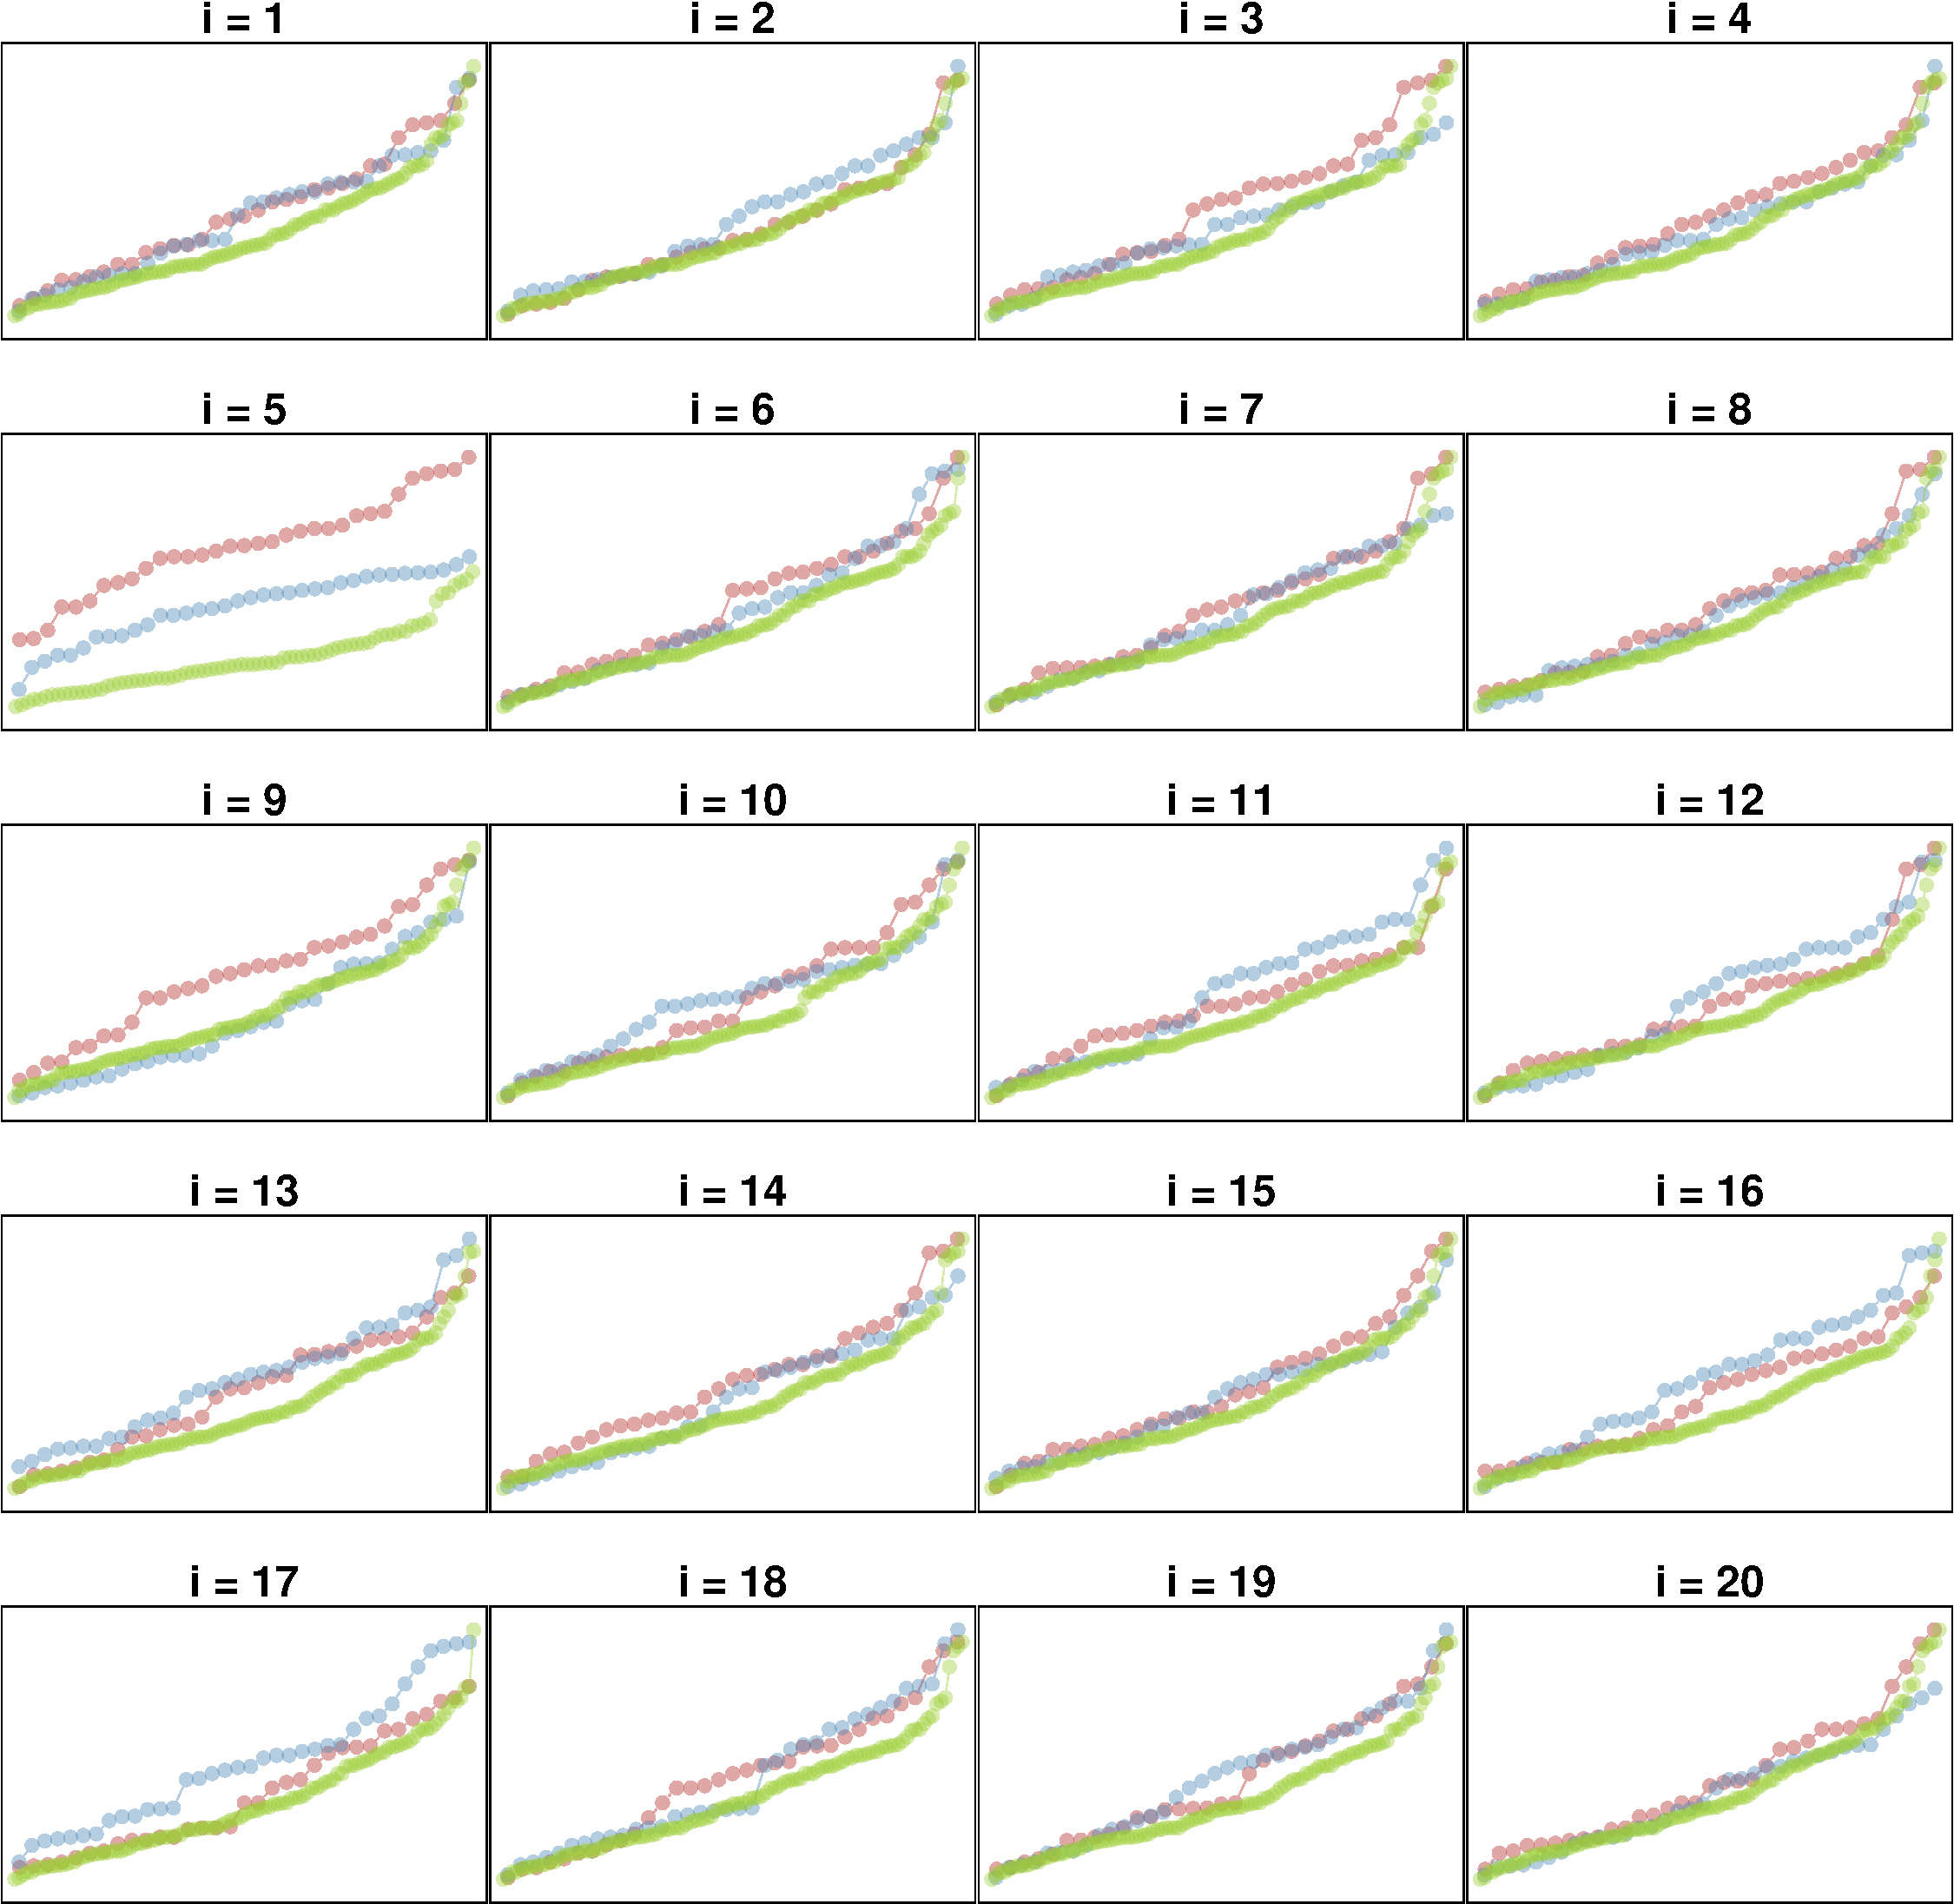
\includegraphics{a4_testing_files/figure-latex/unnamed-chunk-9-1} \end{center}

\begin{verbatim}
## $trueLoc
## [1] "log(6.6790315523026e+66, base=39) - 37"
\end{verbatim}

From the lineup test, it is visually clear that the true plot is at
\(i = 5\) - which is indeed equal to the generated value of
\texttt{trueLoc} - as in this plot, none of the graphs never overlap
unlike every other plot. Hence, using this lineup test, there is enough
evidence to reject the hypothesis that the three sets come from the
same-shaped distribution.

\eenum
\eenum
\eenum


\end{document}
